\documentclass[a4paper,12pt]{article}

% --- Input e lingua ---
\usepackage[utf8]{inputenc}
\usepackage[italian]{babel}

% --- Grafica e font ---
\usepackage{lmodern}           
\usepackage{titlesec}           
\usepackage{fancyhdr}           
\usepackage[table]{xcolor}     
\usepackage{tcolorbox}         
\usepackage{enumitem}           

% --- Matematica e simboli ---
\usepackage{amsmath, amssymb}

% --- Layout pagina ---
\usepackage{geometry}
\geometry{margin=2.5cm}         

% --- Grafica e diagrammi ---
\usepackage{graphicx}           
\usepackage{tikz}              
\usetikzlibrary{shapes.geometric, arrows, positioning, fit, calc, positioning,arrows.meta,shapes}

% --- Link e riferimenti ---
\usepackage{hyperref}

\usepackage{tabularx} % nel preambolo
\usepackage{colortbl} % se usi colori come myblue/mygray

% --- Configurazione link blu e moderni per indice ---
\hypersetup{
    colorlinks=true,
    linkcolor=myblue,
    urlcolor=myblue,
    citecolor=myblue,
    filecolor=myblue,
    pdfborder={0 0 0}
}

\tikzset{
  class/.style={
    rectangle, draw=black, rounded corners,
    minimum width=3.5cm,
    minimum height=1.2cm,
    font=\footnotesize,
    align=left,
    text width=3.5cm,
    inner sep=0.3cm
  },
  % Stili per diverse relazioni UML
  association/.style={thick},
  generalization/.style={-{Triangle[open,length=8pt,width=10pt]}, thick}, 
  dependency/.style={->, thick, dashed}, 
  composition/.style={-{Diamond[fill=black]}, thick},
  aggregation/.style={-{Diamond[open]}, thick}, 
  relation/.style={->, thick}, 
  every node/.style={anchor=center}
}

% --- Miglioramento grafica indice ---
\usepackage{tocloft}
% Colore titoli indice
\renewcommand{\cftsecfont}{\color{myblue}\bfseries}
\renewcommand{\cftsubsecfont}{\color{myblue}}
\renewcommand{\cftsecpagefont}{\color{myblue}\bfseries}
\renewcommand{\cftsubsecpagefont}{\color{myblue}}
% Spaziatura tra voci
\setlength{\cftbeforesecskip}{6pt}
\setlength{\cftbeforesubsecskip}{2pt}

% --- Evidenziazione codice SQL stile editor ---
\usepackage{listings}
\usepackage{color}
\definecolor{editorbg}{RGB}{245,245,250}
\definecolor{sqlblue}{RGB}{0,102,204}
\definecolor{sqlgray}{RGB}{120,120,120}
\definecolor{sqlstring}{RGB}{0,150,0}
\lstdefinestyle{sqlstyle}{
    backgroundcolor=\color{editorbg},
    frame=single,
    rulecolor=\color{myblue},
    language=SQL,
    basicstyle=\ttfamily\small,
    keywordstyle=\color{sqlblue}\bfseries,
    commentstyle=\color{sqlgray}\itshape,
    stringstyle=\color{sqlstring},
    showstringspaces=false,
    breaklines=true,
    tabsize=2
}

% Colori personalizzati
\definecolor{myblue}{RGB}{0, 102, 204}
\definecolor{mygray}{RGB}{240, 240, 240}

% Titoli sezioni colorati e moderni
\titleformat{\section}{\normalfont\Large\bfseries\color{myblue}}{\thesection}{1em}{}
\titleformat{\subsection}{\normalfont\large\bfseries\color{myblue}}{\thesubsection}{1em}{}

% Intestazione e piè di pagina
\pagestyle{fancy}
\setlength{\headheight}{14.5pt}
\fancyhf{}
\fancyhead[L]{\color{myblue}Documentazione Basi di Dati}
\fancyhead[R]{\color{myblue}Gino Pandozzi-Trani}
\fancyfoot[C]{\thepage}

% Elenchi con pallini blu
\setlist[itemize]{label=\textcolor{myblue}{\textbullet}}

\begin{document}

% --- Logo Federico II separato ---
\begin{center}
    
\includegraphics[width=\textwidth]{../Immagini/Federico-II.png}
\end{center}
\vspace{1cm}

% --- Frontespizio migliorato ---
\begin{tcolorbox}[colback=mygray,colframe=myblue,width=\textwidth,arc=6mm,boxrule=1.2pt]
    \begin{center}
        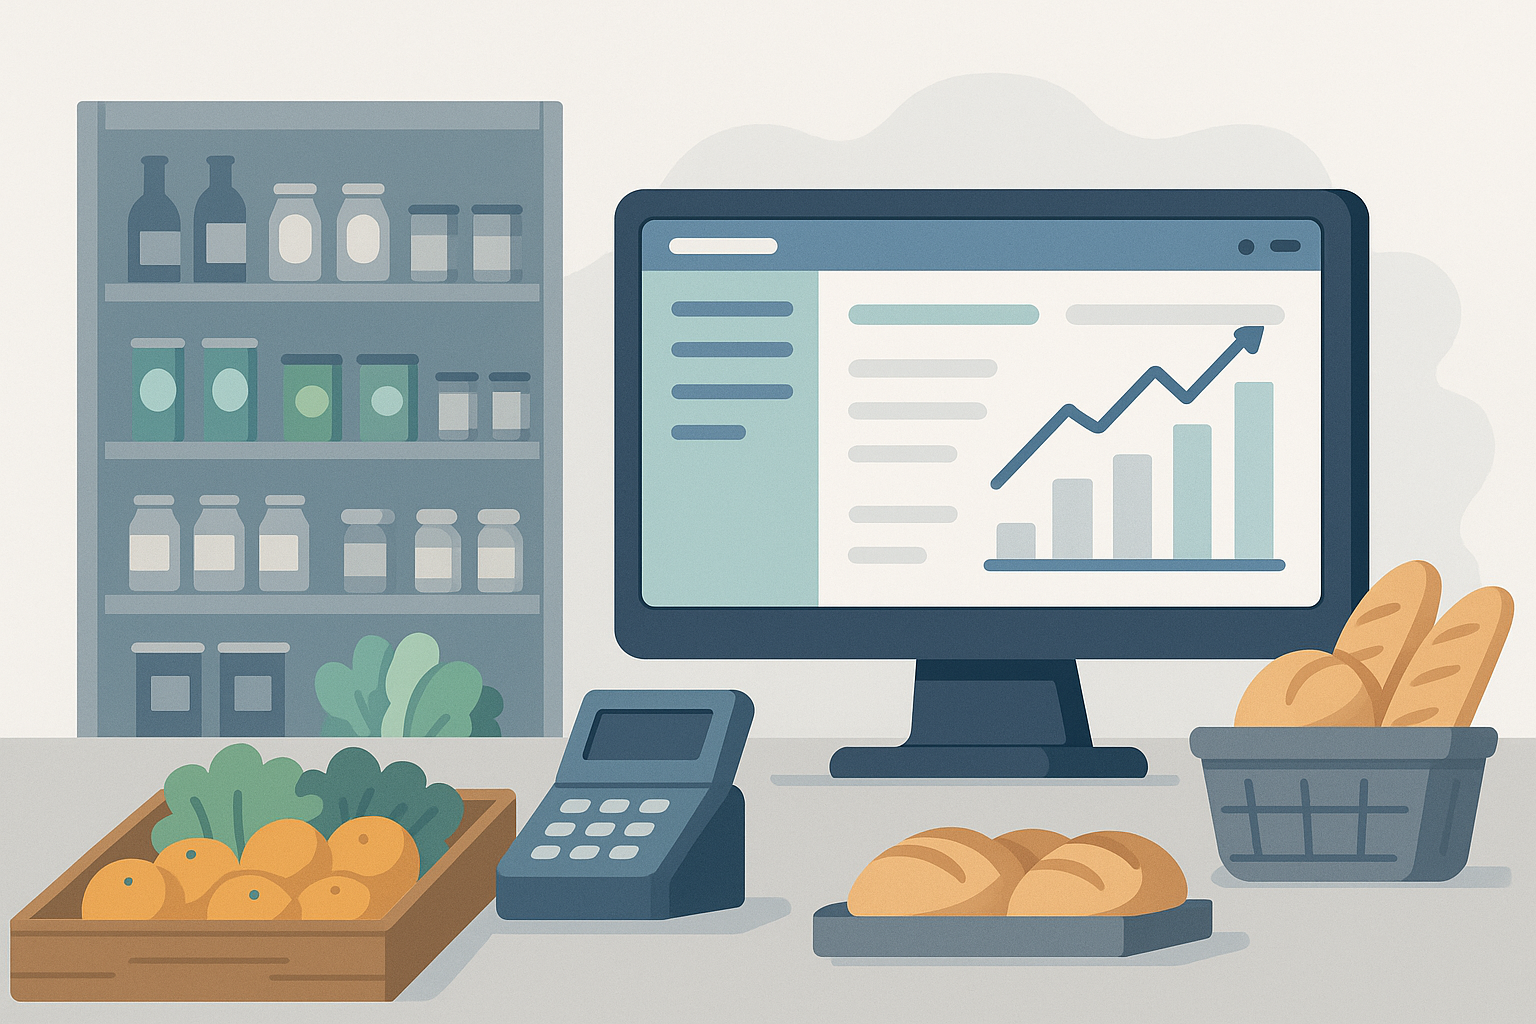
\includegraphics[width=0.6\textwidth]{../Immagini/Frontespazio.png} \\
        \vspace{1cm}
        {\Huge\bfseries\color{myblue} Sistema di Gestione per un Negozio di Alimentari} \\
        \vspace{1cm}
        {\Large\color{black} Autore: Gino Pandozzi-Trani} \\
        \vspace{0.5cm}
    \end{center}
\end{tcolorbox}

\newpage

% Indice racchiuso in box colorato e titolo personalizzato
\begin{tcolorbox}[colback=mygray,colframe=myblue,width=\textwidth,arc=4mm,boxrule=1pt]
    \begin{center}
        {\Huge\bfseries\color{myblue}Indice}
    \end{center}
    \vspace{0.5em}
    \tableofcontents
\end{tcolorbox}

\newpage
\section{Introduzione al Progetto}

\textbf{Sistema di gestione per un negozio di alimentari}

Il presente progetto riguarda lo sviluppo di un sistema informativo per la gestione di un negozio di ortofrutta, con l’obiettivo di supportare in modo efficiente le attività quotidiane del punto vendita.  
Il sistema è pensato per facilitare la gestione delle vendite, del magazzino e dei clienti, fornendo al contempo strumenti per l’analisi delle performance commerciali e l’ottimizzazione dei processi interni.

In particolare, il sistema consente di:
\begin{itemize}
    \item Gestire i prodotti disponibili, classificandoli per tipologia (frutta, verdura, farinacei, latticini, uova e prodotti confezionati), ciascuna caratterizzata da attributi specifici. Ad esempio, la frutta e la verdura sono associate a una data di raccolta, mentre i latticini riportano la data di mungitura e quella di produzione;
    \item Registrare i clienti e gestire le relative tessere punti, calcolando automaticamente i punti fedeltà pari al 10\% del valore di ogni acquisto;
    \item Ricercare i clienti in base ai prodotti acquistati e alla quantità di punti accumulati per ciascuna categoria di prodotto;
    \item Gestire i dipendenti, associando a ciascuna vendita il personale responsabile, con possibilità di analizzare il numero di vendite effettuate e l’introito generato in un determinato periodo.
\end{itemize}

Il progetto si colloca in un contesto accademico volto a sviluppare competenze nella progettazione e realizzazione di sistemi informativi, con particolare attenzione agli aspetti di modellazione dei dati, efficienza operativa e sicurezza delle informazioni.

\newpage
\subsection{Analisi dei Requisiti}

Il sistema deve garantire le seguenti funzionalità principali:
\begin{itemize}
    \item La gestione dei prodotti, classificati per tipologia (frutta, verdura, farinacei, latticini, uova e prodotti confezionati), ognuna dotata di caratteristiche specifiche;
    \item La gestione dei clienti, comprendente la registrazione dei dati personali e delle tessere punti;
    \item La gestione dei dipendenti, con tracciamento delle vendite associate a ciascun membro del personale;
    \item La generazione di statistiche e report, come l’analisi dei clienti in base alle categorie di prodotti acquistati, ai punti fedeltà accumulati e alle performance dei dipendenti;
    \item La tutela dei dati sensibili dei clienti e l’affidabilità delle operazioni quotidiane del negozio.
\end{itemize}

\subsection{Descrizione della Traccia}

\textbf{Traccia 5: Sistema di gestione per un negozio di alimentari}

Il progetto prevede la realizzazione di un sistema informativo per la gestione di un negozio di ortofrutta.  
Il sistema deve consentire di gestire le vendite e la disponibilità dei prodotti, identificando le diverse tipologie merceologiche (frutta, verdura, farinacei, latticini, uova e confezionati). Ogni categoria presenta caratteristiche peculiari: ad esempio, la frutta e la verdura includono la data di raccolta, mentre i latticini riportano sia la data di mungitura del latte sia la data di produzione.

Ogni cliente deve essere registrato nel sistema e disporre di una tessera punti che lo identifichi presso il negozio. Per ogni acquisto effettuato, il cliente accumula punti fedeltà pari al 10\% del valore della spesa.  
Il sistema deve inoltre permettere di ricercare i clienti, distinguendoli in base alle categorie di prodotti acquistati e alla quantità di punti maturati per ciascuna tipologia.

Nel caso in cui siano presenti più dipendenti, ogni vendita deve essere associata al dipendente che l’ha conclusa. Deve pertanto essere possibile individuare, in un determinato intervallo temporale, il dipendente che ha effettuato il maggior numero di vendite e quello che ha generato il più alto introito per il negozio.

\newpage
\section{Progettazione Concettuale}

\subsection{Diagramma ER}
Il \textbf{diagramma Entità--Relazioni (ER)} descrive la struttura logica delle informazioni gestite dal sistema e le interdipendenze tra le sue principali entità. 
Il modello è stato progettato per supportare in modo coerente la gestione degli ordini, dei clienti e dei prodotti, garantendo integrità referenziale e tracciabilità delle transazioni.

Le \textbf{entità principali} individuate sono:
\begin{itemize}
    \item \textbf{CLIENTE}, che rappresenta l’utente che effettua gli acquisti e di cui vengono memorizzati i dati anagrafici e di contatto;
    \item \textbf{TESSERA}, associata univocamente a un cliente, consente di gestire il sistema a punti e il relativo stato operativo (attiva, sospesa, scaduta);
    \item \textbf{ORDINE}, che descrive ciascun acquisto, includendo data, prezzo totale e riferimenti al cliente e al dipendente che lo gestisce;
    \item \textbf{DIPENDENTE}, rappresenta il personale responsabile dell’elaborazione degli ordini;
    \item \textbf{PRODOTTO}, che modella gli articoli in vendita, distinti in categorie merceologiche tramite una specializzazione (\emph{Frutta, Verdura, Latticini}, ecc.);
    \item \textbf{ARTICOLI\_ORDINE}, entità debole che concretizza la relazione molti-a-molti tra \emph{Ordine} e \emph{Prodotto}, includendo le informazioni quantitative e di prezzo.
\end{itemize}

Le \textbf{relazioni} principali sono:
\begin{itemize}
    \item \emph{possiede}, tra \textbf{Cliente} e \textbf{Tessera} (1:1);
    \item \emph{effettua}, tra \textbf{Cliente} e \textbf{Ordine} (1:N);
    \item \emph{gestisce}, tra \textbf{Dipendente} e \textbf{Ordine} (1:N);
    \item \emph{contiene}, tra \textbf{Ordine} e \textbf{Prodotto} (N:M, tramite \textbf{Articoli\_Ordine}).
\end{itemize}

Questo schema ER consente di rappresentare in modo completo i vincoli semantici del dominio, predisponendo la base per la successiva progettazione logica del database relazionale.


\begin{center}
\begin{tikzpicture}[
    entity/.style={
      rectangle, draw=black, thick,
      minimum width=2cm, minimum height=0.7cm,
      fill=teal!30, font=\scriptsize\bfseries, rounded corners=2pt
    },
    weakentity/.style={
      rectangle, draw=black, thick, double, double distance=1pt, double=teal!30,
      minimum width=2cm, minimum height=0.7cm, fill=teal!30,
      font=\scriptsize\bfseries, rounded corners=2pt
    },
    attribute/.style={
      ellipse, draw=black, minimum width=1cm, minimum height=0.5cm,
      fill=teal!20, font=\tiny
    },
    key/.style={
      ellipse, draw=black, minimum width=1cm, minimum height=0.5cm,
      fill=teal!20, font=\tiny\bfseries
    },
    relationship/.style={
      diamond, draw=black, thick, minimum width=1.5cm, minimum height=0.7cm,
      fill=yellow!60, font=\scriptsize\bfseries
    },
    node distance=0.8cm and 1.2cm,
    scale=0.85, transform shape
]

% =============================
% CLIENTE
% =============================
\node[entity] (cliente) at (-8,8) {CLIENTE};
\node[key, above=0.6cm of cliente] (codcliente) {\underline{codcliente}};
\node[attribute, above left=0.6cm and 0.8cm of cliente] (nome_c) {nome};
\node[attribute, above right=0.6cm and 0.8cm of cliente] (cognome_c) {cognome};
\node[attribute, left=0.9cm of cliente] (cf_c) {codicefiscale};
\node[attribute, below left=1.0cm and -0.2cm of cliente] (indirizzo_c) {indirizzo};
\node[attribute, below left=0.4cm and 1.0cm of cliente] (telefono_c) {telefono};
\node[attribute, below right=0.6cm and 0.8cm of cliente] (email_c) {email};

% Relazione POSSIEDE
\node[relationship] (possiede) at (-2,8) {possiede};

% =============================
% TESSERA
% =============================
\node[entity] (tessera) at (4.5,8) {TESSERA};
\node[key, above=0.6cm of tessera] (codtessera) {\underline{codtessera}};
\node[attribute, above left=0.6cm and 0.8cm of tessera] (numeropunti) {numeropunti};
\node[attribute, above right=0.6cm and 0.8cm of tessera] (dataemissione) {dataemissione};
\node[attribute, right=0.9cm of tessera] (datascadenza) {datascadenza};
\node[ellipse, draw=black, double, double distance=1pt, double=teal!30,
      line width=0.8pt, fill=teal!30, minimum width=1.5cm, minimum height=0.6cm,
      below=1.0cm of tessera, font=\scriptsize] (statotessera) {statotessera};

% =============================
% ORDINE
% =============================
\node[relationship] (effettua) at (-8,4.5) {effettua};
\node[entity] (ordine) at (-8,1) {ORDINE};
\node[attribute, above left=0.6cm and 0.8cm of ordine] (dataacquisto) {dataacquisto};
\node[attribute, left=0.9cm of ordine] (prezzototale) {prezzototale};
\node[key, below=0.6cm of prezzototale] (codordine) {\underline{codordine}};

% =============================
% DIPENDENTE
% =============================
\node[entity] (dipendente) at (-8,-6) {DIPENDENTE};
\node[attribute, above left=0.6cm and 0.8cm of dipendente] (nome_d) {nome};
\node[attribute, above right=0.6cm and 0.8cm of dipendente] (cognome_d) {cognome};
\node[attribute, left=0.9cm of dipendente] (cf_d) {codicefiscale};
\node[attribute, right=0.9cm of dipendente] (indirizzo_d) {indirizzo};
\node[attribute, below left=0.6cm and 0.8cm of dipendente] (telefono_d) {telefono};
\node[attribute, below right=0.6cm and 0.8cm of dipendente] (email_d) {email};
\node[key, below=0.6cm of dipendente] (coddipendente) {\underline{coddipendente}};

\node[relationship] (gestisce) at (-8,-2.5) {gestisce};

% =============================
% ARTICOLI_ORDINE (entità debole)
% =============================
\node[weakentity] (articoli_ordine) at (0,1) {ARTICOLI\_ORDINE};
\node[attribute, below right=0.6cm and 0.8cm of articoli_ordine] (prezzo_art) {prezzo};
\node[attribute, right=0.9cm of articoli_ordine] (numeroarticoli) {numeroarticoli};

% =============================
% PRODOTTO + specializzazione
% =============================
\node[entity] (prodotto) at (3.5,-6) {PRODOTTO};
\node[key, below=1.0cm of prodotto] (codprodotto) {\underline{codprodotto}};
\node[attribute, above left=0.6cm and 1.0cm of prodotto] (nome_p) {nome};
\node[attribute, above right=0.6cm and 1.0cm of prodotto] (descrizione) {descrizione};
\node[attribute, left=1.3cm of prodotto] (prezzo_p) {prezzo};
\node[attribute, right=1.3cm of prodotto] (luogoprovenienza) {luogoprovenienza};
\node[attribute, above=0.8cm of prodotto] (scorta) {scorta};

% Nodo specializzazione
\node[draw, circle, minimum size=0.4cm, fill=teal!30, double, double distance=1pt, double=teal!30] (spec_prod) at (-2,-10) {\textbf{d}};

% Figli specializzazione
\node[entity] (frutta) at (-11,-14) {FRUTTA};
\node[attribute, below=0.6cm of frutta] (dataraccolta_f) {dataraccolta};

\node[entity] (verdura) at (-8,-14) {VERDURA};
\node[attribute, below=0.6cm of verdura] (dataraccolta_v) {dataraccolta};

\node[entity] (confezionati) at (-5,-14) {CONFEZIONATI};
\node[attribute, below=0.6cm of confezionati] (datascadenza_c) {datascadenza};

\node[entity] (farinacei) at (-2,-14) {FARINACEI};
\node[attribute, below=0.6cm of farinacei] (glutine_fa) {glutine};

\node[entity] (uova) at (1,-14) {UOVA};
\node[attribute, below=0.6cm of uova] (datascadenza_u) {datascadenza};

\node[entity] (latticini) at (4,-14) {LATTICINI};
\node[attribute, above right=0.6cm and 0.6cm of latticini] (datamungitura_l) {datamungitura};
\node[attribute, below right=0.6cm and 0.6cm of latticini] (dataproduzione_l) {dataproduzione};
\node[attribute, below=1.0cm of latticini] (datascadenza_l) {datascadenza};

% Connessioni (stesso codice originale)
\draw (cliente) -- (codcliente);
\draw (cliente) -- (nome_c);
\draw (cliente) -- (cognome_c);
\draw (cliente) -- (cf_c);
\draw (cliente) -- (indirizzo_c);
\draw (cliente) -- (telefono_c);
\draw (cliente) -- (email_c);

\draw (tessera) -- (codtessera);
\draw (tessera) -- (numeropunti);
\draw (tessera) -- (dataemissione);
\draw (tessera) -- (datascadenza);
\draw (tessera) -- (statotessera);

\draw (dipendente) -- (coddipendente);
\draw (dipendente) -- (nome_d);
\draw (dipendente) -- (cognome_d);
\draw (dipendente) -- (cf_d);
\draw (dipendente) -- (indirizzo_d);
\draw (dipendente) -- (telefono_d);
\draw (dipendente) -- (email_d);

\draw (prodotto) -- (codprodotto);
\draw (prodotto) -- (nome_p);
\draw (prodotto) -- (descrizione);
\draw (prodotto) -- (prezzo_p);
\draw (prodotto) -- (luogoprovenienza);
\draw (prodotto) -- (scorta);

\draw[thick] (prodotto) -- (spec_prod);

\draw[thick] (spec_prod) -- node[midway, sloped] {$\rotatebox[origin=c]{-90}{$\cup$}$} (frutta);
\draw[thick] (spec_prod) -- node[midway, sloped] {$\rotatebox[origin=c]{-90}{$\cup$}$} (verdura);
\draw[thick] (spec_prod) -- node[midway, sloped] {$\rotatebox[origin=c]{-90}{$\cup$}$} (confezionati);
\draw[thick] (spec_prod) -- node[midway, sloped] {$\rotatebox[origin=c]{-90}{$\cup$}$} (farinacei);
\draw[thick] (spec_prod) -- node[midway, sloped] {$\rotatebox[origin=c]{90}{$\cup$}$} (uova);
\draw[thick] (spec_prod) -- node[midway, sloped] {$\rotatebox[origin=c]{90}{$\cup$}$} (latticini);

\draw (frutta) -- (dataraccolta_f);
\draw (verdura) -- (dataraccolta_v);
\draw (confezionati) -- (datascadenza_c);
\draw (farinacei) -- (glutine_fa);
\draw (uova) -- (datascadenza_u);
\draw (latticini) -- (datamungitura_l);
\draw (latticini) -- (dataproduzione_l);
\draw (latticini) -- (datascadenza_l);

\draw (ordine) -- (codordine);
\draw (ordine) -- (prezzototale);
\draw (ordine) -- (dataacquisto);

\draw (articoli_ordine) -- (prezzo_art);
\draw (articoli_ordine) -- (numeroarticoli);

\draw[thick] (cliente) -- (possiede) -- (tessera);
\draw[thick] (cliente) -- (effettua) -- (ordine);
\draw[thick] (dipendente) -- (gestisce) -- (ordine);
\draw[thick] (ordine) -- (articoli_ordine) -- (prodotto);

\end{tikzpicture}
\end{center}

\subsection{Diagramma Concettuale}
Il \textbf{diagramma concettuale} riformula il modello ER in termini di classi e relazioni, secondo una prospettiva orientata agli oggetti. 
Tale rappresentazione evidenzia la struttura semantica dei dati e le relazioni logiche tra le entità, favorendo la successiva transizione verso il modello logico o implementativo (ad esempio in UML o in codice).

In particolare:
\begin{itemize}
    \item \textbf{Persona} è una \emph{superclasse astratta} che raccoglie gli attributi comuni a \textbf{Cliente} e \textbf{Dipendente}, riducendo la ridondanza informativa;
    \item \textbf{Cliente} e \textbf{Dipendente} derivano da \textbf{Persona} ed estendono la classe con un proprio identificativo univoco;
    \item \textbf{Ordine} funge da nodo centrale tra \textbf{Cliente} e \textbf{Dipendente}, rappresentando la transazione commerciale e mantenendo le associazioni con i prodotti acquistati;
    \item \textbf{ArticoliOrdine} è una \emph{classe di associazione} tra \textbf{Ordine} e \textbf{Prodotto}, contenente il prezzo unitario e la quantità;
    \item \textbf{Prodotto} è una classe generalizzata che comprende diverse specializzazioni (\emph{Frutta, Verdura, Latticini}, ecc.), ciascuna con attributi specifici coerenti con la categoria merceologica.
\end{itemize}

Questo modello concettuale consente una visione più astratta e modulare dei dati, facilitando l’estensione del dominio e la successiva mappatura su schemi relazionali o classi software.

\begin{center}
\resizebox{\textwidth}{!}{%
\begin{tikzpicture}[node distance=3.2cm and 5.2cm, transform shape]

% Livello superiore - Persona come entità principale (centrale)
\node[class] (persona) at (0,0) {
  \textbf{Persona}\\[-0.3em]\rule{\linewidth}{0.2pt}\\
  + nome : string\\
  + cognome : string\\
  + codicefiscale : string\\
  + indirizzo : string\\
  + telefono : string\\
  + email : string
};

% Livello secondo - Specializzazioni di Persona (più distanziate)
\node[class] (cliente) at (-7,-3.5) {
  \textbf{Cliente}\\[-0.3em]\rule{\linewidth}{0.2pt}\\
  + codcliente : int
};

\node[class] (dipendente) at (7,-3.5) {
  \textbf{Dipendente}\\[-0.3em]\rule{\linewidth}{0.2pt}\\
  + coddipendente : int
};

% Livello terzo - Entità collegate a Cliente (allineate sotto cliente)
\node[class] (tessera) at (-7,-8) {
  \textbf{Tessera}\\[-0.3em]\rule{\linewidth}{0.2pt}\\
  + codtessera : int\\
  + codcliente : int\\
  + numeropunti : numeric\\
  + dataemissione : date\\
  + datascadenza : date\\
  + stato : STATOTESSERA
};

% Livello centrale - Ordine come entità di collegamento
\node[class] (ordine) at (0,-8) {
  \textbf{Ordine}\\[-0.3em]\rule{\linewidth}{0.2pt}\\
  + codordine : int\\
  + prezzototale : real\\
  + dataacquisto : date\\
  + codcliente : int\\
  + coddipendente : int
};

% Livello quarto - ArticoliOrdine
\node[class] (articoli) at (0,-12) {
  \textbf{ArticoliOrdine}\\[-0.3em]\rule{\linewidth}{0.2pt}\\
  + codordine : int\\
  + codprodotto : int\\
  + prezzo : numeric\\
  + numeroarticoli : int
};

% Livello destro - Prodotto e sue specializzazioni (spostato più a destra)
\node[class] (prodotto) at (12,-8) {
  \textbf{Prodotto}\\[-0.3em]\rule{\linewidth}{0.2pt}\\
  + codprodotto : int\\
  + nome : string\\
  + descrizione : string\\
  + prezzo : numeric\\
  + luogoprovenienza : string\\
  + scorta : int
};

% Specializzazioni di Prodotto - disposte simmetricamente
% Specializzazioni di Prodotto - frutta in basso
\node[class] (frutta) at (2,-15) {
  \textbf{Frutta}\\[-0.3em]\rule{\linewidth}{0.2pt}\\
  + dataraccolta : date
};

% Specializzazioni di Prodotto - verdura in alto a destra
\node[class] (verdura) at (17,-10) {
  \textbf{Verdura}\\[-0.3em]\rule{\linewidth}{0.2pt}\\
  + dataraccolta : date
};

% Specializzazioni di Prodotto - latticini in basso
\node[class] (latticini) at (8,-15) {
  \textbf{Latticini}\\[-0.3em]\rule{\linewidth}{0.2pt}\\
  + datamungitura : date\\
  + dataproduzione : date\\
  + datascadenza : date
};

% Specializzazioni di Prodotto - farinacei in alto a destra
\node[class] (farinacei) at (17,-13) {
  \textbf{Farinacei}\\[-0.3em]\rule{\linewidth}{0.2pt}\\
  + glutine : boolean
};

% Specializzazioni di Prodotto - uova in basso
\node[class] (uova) at (14,-15) {
  \textbf{Uova}\\[-0.3em]\rule{\linewidth}{0.2pt}\\
  + datascadenza : date
};

% Specializzazioni di Prodotto - confezionati in alto a destra
\node[class] (confezionati) at (17,-7) {
  \textbf{Confezionati}\\[-0.3em]\rule{\linewidth}{0.2pt}\\
  + datascadenza : date
};

% Relazioni principali - Ereditarietà (generalizzazione)
\draw[generalization] (cliente) -- (persona);
\draw[generalization] (dipendente) -- (persona);

% Relazioni Cliente 
\draw[composition] (cliente) -- node[midway, left] {possiede} node[near start, right] {1} node[near end, right] {1} (tessera);
\draw[association] (cliente) -- node[midway, right] {effettua} node[near start, left] {1} node[near end, left] {*} (ordine);

% Relazioni Dipendente
\draw[association] (dipendente) -- node[midway, right] {gestisce} node[near start, left] {1} node[near end, left] {*} (ordine);

% Relazioni Ordine-ArticoliOrdine-Prodotto
\draw[composition] (ordine) -- node[midway, right] {contiene} node[near start, left] {1} node[near end, left] {*} (articoli);
\draw[association] (articoli) -- node[midway, right] {riferisce} node[near start, right] {*} node[near end, above] {1} (prodotto);

% Generalizzazioni Prodotto - con triangoli di generalizzazione
\draw[generalization] (frutta) -- (prodotto);
\draw[generalization] (verdura) -- (prodotto);
\draw[generalization] (latticini) -- (prodotto);
\draw[generalization] (farinacei) -- (prodotto);
\draw[generalization] (uova) -- (prodotto);
\draw[generalization] (confezionati) -- (prodotto);

\end{tikzpicture}
} % fine resizebox
\end{center}

\subsection{Diagramma Concettuale Ristrutturato}

Il \textbf{diagramma concettuale ristrutturato} rappresenta una versione ottimizzata e normalizzata del modello concettuale precedente. 
L’obiettivo della ristrutturazione è ridurre la complessità derivante dalla presenza di numerose specializzazioni, accorpando le categorie di prodotti in un’unica classe più flessibile e parametrizzata.

\begin{itemize}
\item La \textbf{classe \texttt{Prodotto}} è stata unificata e arricchita con un attributo enumerativo \texttt{categoria}, che consente di distinguere le diverse tipologie di articoli. Gli attributi specifici (ad esempio \emph{data raccolta}, \emph{data mungitura}, \emph{data scadenza}, \emph{presenza glutine}) sono ora integrati nella stessa classe e possono assumere valore nullo quando non pertinenti alla tipologia di prodotto. Questa scelta riduce la complessità del modello e favorisce una maggiore flessibilità nella gestione dei dati;

\item Le classi \textbf{Cliente} e \textbf{Dipendente} sono state accorpate nella \textbf{superclasse \texttt{Persona}}, dalla quale ereditano gli attributi comuni (come \emph{nome}, \emph{cognome}, \emph{codice fiscale}, \emph{indirizzo}, \emph{telefono} ed \emph{email}). Tale ristrutturazione migliora la coerenza semantica e semplifica la gestione delle relazioni con le altre entità, mantenendo la distinzione logica tra clienti e dipendenti;

\item Le relazioni tra \textbf{Cliente}, \textbf{Tessera}, \textbf{Ordine} e \textbf{ArticoliOrdine} sono state mantenute inalterate, poiché già correttamente rispecchiano i vincoli cardinali e semantici del dominio applicativo, garantendo la tracciabilità e l’integrità delle transazioni;

\item Sono state introdotte \textbf{enumerazioni} (come \texttt{STATOTESSERA} e \texttt{TIPOLOGIA}) per rappresentare domini discreti e garantire coerenza, validità e uniformità dei valori nei dati, facilitando al contempo i controlli di integrità a livello applicativo e di database.
\end{itemize}

Questa versione del modello risulta più compatta e facilmente traducibile in un modello relazionale normalizzato, mantenendo al contempo l’integrità semantica e la chiarezza del design concettuale.

\begin{center}
\resizebox{\textwidth}{!}{%
\begin{tikzpicture}[node distance=3.2cm and 5.2cm, transform shape]

% Livello superiore - Cliente e Dipendente affiancati (più distanziati)
\node[class] (cliente2) at (-7,0) {
  \textbf{Cliente}\\[-0.3em]\rule{\linewidth}{0.2pt}\\
  + codcliente : int\\
  + nome : string\\
  + cognome : string\\
  + codicefiscale : string\\
  + indirizzo : string\\
  + telefono : string\\
  + email : string
};

\node[class] (dipendente2) at (7,0) {
  \textbf{Dipendente}\\[-0.3em]\rule{\linewidth}{0.2pt}\\
  + coddipendente : int\\
  + nome : string\\
  + cognome : string\\
  + codicefiscale : string\\
  + indirizzo : string\\
  + telefono : string\\
  + email : string
};

% Livello secondo - Tessera e Ordine (più distanziati)
\node[class] (tessera2) at (-11,-6.5) {
  \textbf{Tessera}\\[-0.3em]\rule{\linewidth}{0.2pt}\\
  + codtessera : int\\
  + codcliente : int\\
  + numeropunti : numeric\\
  + dataemissione : date\\
  + datascadenza : date\\
  + stato : STATOTESSERA
};

\node[class] (ordine2) at (0,-6.5) {
  \textbf{Ordine}\\[-0.3em]\rule{\linewidth}{0.2pt}\\
  + codordine : int\\
  + prezzototale : real\\
  + dataacquisto : date\\
  + codcliente : int\\
  + coddipendente : int
};

% Livello terzo - Prodotto a destra (più largo e distanziato)
\node[class] (prodotto2) at (0,-21) {
  \textbf{Prodotto}\\[-0.3em]\rule{\linewidth}{0.2pt}\\
  + codprodotto : int\\
  + nome : string\\
  + descrizione : string\\
  + prezzo : numeric\\
  + luogoprovenienza : string\\
  + dataraccolta : date\\
  + datamungitura : date\\
  + glutine : boolean\\
  + datascadenza : date\\
  + dataproduzione : date\\
  + categoria : {FRUTTA, VERDURA, LATTICINI, FARINACEI, UOVA, CONFEZIONATI}\\
  + scorta : int
};

% Livello inferiore - ArticoliOrdine al centro (più in basso)
\node[class] (articoli2) at (0,-11.5) {
  \textbf{ArticoliOrdine}\\[-0.3em]\rule{\linewidth}{0.2pt}\\
  + codordine : int\\
  + codprodotto : int\\
  + prezzo : numeric\\
  + numeroarticoli : int
};

% Enumerazioni - posizionate sotto le rispettive entità
\node[class] (statotessera) at (-11,-11) {
  \textbf{«enumeration»}\\
  \textbf{STATOTESSERA}\\[-0.3em]\rule{\linewidth}{0.2pt}\\
  ATTIVA\\
  SOSPESA\\
  SCADUTA
};

\node[class] (tipologia) at (5,-19) {
  \textbf{«enumeration»}\\
  \textbf{TIPOLOGIA}\\[-0.3em]\rule{\linewidth}{0.2pt}\\
  FRUTTA\\
  VERDURA\\
  FARINACEI\\
  LATTICINI\\
  UOVA\\
  CONFEZIONATI
};

% Relazioni con etichette descrittive
\draw[composition] (cliente2) -- node[pos=0.6, left] {possiede} node[near start, right] {1} node[near end, right] {1} (tessera2);
\draw[association] (cliente2) -- node[pos=0.5, right] {effettua} node[near start, left] {1} node[near end, left] {*} (ordine2);
\draw[association] (dipendente2) -- node[pos=0.5, left] {gestisce} node[near start, right] {1} node[near end, right] {*} (ordine2);
\draw[composition] (ordine2) -- node[midway, right] {contiene} node[near start, left] {1} node[near end, left] {*} (articoli2);
\draw[association] (articoli2) -- node[midway, right] {riferisce} node[near start, right] {*} node[near end, right] {1} (prodotto2);

% Dipendenze per le enumerazioni (linee tratteggiate)
%\draw[dependency] (tessera2) -- node[pos=0.7, right] {«uses»} (statotessera);
%\draw[dependency] (prodotto2) -- node[pos=0.7, left] {«uses»} (tipologia);

\end{tikzpicture}
} % fine resizebox
\end{center}

\newpage
\section{Progettazione Logica}

\subsection{Schema relazionale}

Lo schema relazionale del database è stato progettato per soddisfare le esigenze di gestione di un negozio di alimentari, garantendo coerenza, integrità dei dati e facilità di interrogazione.  
Sono stati definiti tipi enumerativi per le categorie di prodotto (\texttt{TIPOLOGIA}) e per lo stato della tessera fedeltà (\texttt{STATOTESSERA}), assicurando validazione e chiarezza semantica.  

Le principali entità (\texttt{cliente}, \texttt{tessera}, \texttt{dipendente}, \texttt{prodotto}, \texttt{ordine}, \texttt{articoliordine}) sono state implementate con vincoli di unicità, integrità referenziale e regole di business.  
In particolare, la tabella \texttt{prodotto} include un vincolo \texttt{CHECK} avanzato per garantire che ogni categoria valorizzi solo gli attributi pertinenti, riducendo errori di inserimento.

\textbf{Note progettuali aggiuntive:}
\begin{itemize}
    \item Le chiavi esterne sono definite con \texttt{ON UPDATE CASCADE} per propagare eventuali modifiche dei codici primari.
    \item Alcune FK, come in \texttt{ordine}, hanno \texttt{ON DELETE RESTRICT} per evitare cancellazioni involontarie di clienti o dipendenti collegati ad ordini.
    \item Il tipo \texttt{NUMERIC} è utilizzato per prezzi e punti per garantire precisione decimale e correttezza nei calcoli.
\end{itemize}

\vspace{0.5em}
\renewcommand{\arraystretch}{1.35}
\arrayrulecolor{myblue}
\begin{table}[ht]
\centering
\setlength{\tabcolsep}{8pt}
\begin{tabular}{|>{\centering\arraybackslash}m{3.5cm}|>{\raggedright\arraybackslash}m{10.5cm}|}
\hline
\rowcolor{myblue}\textcolor{white}{\textbf{Tabella}} & \textcolor{white}{\textbf{Attributi principali}} \\
\hline
\rowcolor{mygray} cliente & \underline{codcliente} (PK, SERIAL), nome, cognome, codicefiscale, indirizzo, telefono, email \\
tessera & \underline{codtessera} (PK, SERIAL), \underline{\underline{codcliente}} (FK, UNIQUE), numeropunti, dataemissione, datascadenza, stato \\
\rowcolor{mygray} dipendente & \underline{coddipendente} (PK, SERIAL), nome, cognome, codicefiscale, indirizzo, telefono, email \\
prodotto & \underline{codprodotto} (PK, SERIAL), nome, descrizione, prezzo, luogoprovenienza, dataraccolta, datamungitura, glutine, datascadenza, dataproduzione, categoria, scorta \\
\rowcolor{mygray} ordine & \underline{codordine} (PK, SERIAL), prezzototale, dataacquisto, \underline{\underline{codcliente}} (FK), \underline{\underline{coddipendente}} (FK) \\
articoliordine & \underline{codordine} (PK, FK), \underline{codprodotto} (PK, FK), prezzo, numeroarticoli \\
\hline
\end{tabular}
\caption{Schema relazionale: chiavi primarie sottolineate, chiavi esterne doppiamente sottolineate.}
\end{table}
\arrayrulecolor{black}

\subsection{Dizionario delle entità}

Ogni tabella rappresenta un elemento chiave del sistema, con attributi principali e vincoli di integrità:

\begin{itemize}
    \item \textbf{cliente}: dati anagrafici dei clienti, validati tramite regex per email e codice fiscale. Chiave primaria \texttt{codcliente}.  
    \item \textbf{tessera}: tessera punti associata a ciascun cliente (1:1), con saldo punti, stato e date di emissione e scadenza. Chiave primaria \texttt{codtessera}, FK su \texttt{cliente}.  
    \item \textbf{dipendente}: dati anagrafici dei dipendenti, con validazione dei campi. Chiave primaria \texttt{coddipendente}.  
    \item \textbf{prodotto}: prodotti in vendita, con tipologia, attributi specifici per categoria, prezzo e scorta disponibile. Chiave primaria \texttt{codprodotto}. Vincolo \texttt{CHECK} avanzato per coerenza categorie.  
    \item \textbf{ordine}: registra ogni vendita, collegata a cliente e dipendente. Chiave primaria \texttt{codordine}, FK su \texttt{cliente} e \texttt{dipendente}.  
    \item \textbf{articoliordine}: dettaglio dei prodotti acquistati per ogni ordine, con prezzo e quantità. PK composita (\texttt{codordine, codprodotto}), FK su \texttt{ordine} e \texttt{prodotto}.
\end{itemize}

\vspace{0.5em}
\renewcommand{\arraystretch}{1.3}
\arrayrulecolor{myblue}
\begin{table}[htbp]
\centering
\setlength{\tabcolsep}{8pt}
\begin{tabular}{|>{\centering\arraybackslash}m{3.5cm}|>{\raggedright\arraybackslash}m{9.5cm}|}
\hline
\rowcolor{myblue}\textcolor{white}{\textbf{Entità}} & \textcolor{white}{\textbf{Descrizione}} \\
\hline
\rowcolor{mygray} cliente & Dati anagrafici dei clienti, con PK \texttt{codcliente} e validazioni su codice fiscale e email. \\
tessera & Tessera punti (1:1) per cliente, con saldo punti, date di emissione/scadenza e stato. \\
\rowcolor{mygray} dipendente & Dati anagrafici dei dipendenti, PK \texttt{coddipendente}, con validazione dei campi. \\
prodotto & Prodotti in vendita, con tipologia, caratteristiche specifiche, prezzo e scorta, vincolo \texttt{CHECK} avanzato per categorie. \\
\rowcolor{mygray} ordine & Rappresenta una vendita, collegata a cliente e dipendente, con calcolo automatico del prezzo totale. \\
articoliordine & Dettaglio degli articoli per ordine, con prezzo unitario e quantità, PK composita \texttt{(codordine, codprodotto)}. \\
\hline
\end{tabular}
\caption{Entità principali e loro funzione nel database.}
\end{table}
\arrayrulecolor{black}

\subsection{Associazioni e relazioni}

Le relazioni tra entità sono implementate tramite chiavi esterne e vincoli di integrità referenziale:

\begin{itemize}
    \item \textbf{Cliente-Tessera} (1:1): ogni cliente possiede una sola tessera. FK con \texttt{ON DELETE CASCADE}.
    \item \textbf{Ordine-Cliente} (N:1): ogni ordine è associato a un cliente. FK con \texttt{ON DELETE RESTRICT} per protezione dati.
    \item \textbf{Ordine-Dipendente} (N:1): ogni ordine è gestito da un dipendente.
    \item \textbf{Ordine-Prodotto} (N:M): ogni ordine può contenere più prodotti tramite \texttt{articoliordine}.
\end{itemize}

\vspace{0.5em}
\renewcommand{\arraystretch}{1.3}
\arrayrulecolor{myblue}
\begin{table}[htbp]
\centering
\setlength{\tabcolsep}{8pt}
\begin{tabular}{|>{\centering\arraybackslash}m{3.5cm}|>{\raggedright\arraybackslash}m{9.5cm}|}
\hline
\rowcolor{myblue}\textcolor{white}{\textbf{Associazione}} & \textcolor{white}{\textbf{Descrizione}} \\
\hline
\rowcolor{mygray} Cliente-Tessera & Ogni cliente ha una tessera (1:1), FK con \texttt{ON DELETE CASCADE}. \\
Ordine-Cliente & Ogni ordine è associato a un cliente (N:1), FK con \texttt{ON DELETE RESTRICT}. \\
\rowcolor{mygray} Ordine-Dipendente & Ogni ordine è gestito da un dipendente (N:1), FK con \texttt{ON DELETE RESTRICT}. \\
Ordine-Prodotto & Ogni ordine contiene più prodotti tramite \texttt{articoliordine} (N:M). \\
\hline
\end{tabular}
\caption{Principali associazioni tra le entità.}
\end{table}
\arrayrulecolor{black}

\subsection{Vincoli di integrità}

Il database implementa vincoli completi per garantire la coerenza e la qualità dei dati:

\begin{itemize}
    \item Vincoli \texttt{PRIMARY KEY} e \texttt{UNIQUE} per garantire l’unicità dei record.
    \item Vincoli \texttt{FOREIGN KEY} per l’integrità referenziale tra le tabelle.
    \item Vincoli \texttt{CHECK} su valori numerici (\texttt{prezzo $\geq$ 0}, \texttt{scorta $\geq$ 0}), validazione di email e codice fiscale tramite regex.
    \item Vincolo \texttt{CHECK} su \texttt{prodotto} per garantire coerenza attributi/categoria.
    \item Trigger e funzioni associate per:
    \begin{itemize}
        \item Aggiornamento automatico della scorta e dei punti tessera (\texttt{AggiornaScortaEPunti}).
        \item Aggiornamento del prezzo totale dell'ordine (\texttt{AggiornaPrezzoOrdine}, \texttt{AggiornaPrezzoOrdineDelete}).
        \item Verifica della disponibilità della scorta (\texttt{VerificaScortaProdotto}).
        \item Aggiornamento dello stato della tessera (\texttt{AggiornaStatoTessera}).
        \item Ripristino scorta e punti dopo cancellazione articoli ordine (\texttt{RipristinaScortaProdotto}).
    \end{itemize}
\end{itemize}

\vspace{0.5em}
\renewcommand{\arraystretch}{1.3}
\arrayrulecolor{myblue}
\begin{table}[ht]
\centering
\setlength{\tabcolsep}{8pt}
\begin{tabular}{|>{\centering\arraybackslash}m{4cm}|>{\raggedright\arraybackslash}m{10cm}|}
\hline
\rowcolor{myblue}\textcolor{white}{\textbf{Vincolo / Trigger}} & \textcolor{white}{\textbf{Descrizione}} \\
\hline
\rowcolor{mygray} Email Regex & Validazione degli indirizzi email dei clienti e dipendenti. \\
Codice Fiscale Regex & Validazione secondo il formato italiano standard. \\
\rowcolor{mygray} Chiavi Primarie & Unicità dei record in ogni tabella. \\
Chiavi Esterne & Integrità referenziale tra tabelle correlate. \\
\rowcolor{mygray} Vincoli CHECK & Controlli su valori numerici e coerenza attributi per categoria prodotto. \\
Trigger e Funzioni & Gestione automatica di scorte, punti tessera, prezzo ordine e stato tessera. \\
\hline
\end{tabular}
\caption{Vincoli di integrità e regole di business implementati nel database.}
\end{table}
\arrayrulecolor{black}

\newpage
\subsection{Schema logico di funzioni e trigger}

La tabella seguente descrive la logica operativa che governa l'interazione tra le \textbf{tabelle}, le \textbf{funzioni in PL/pgSQL} e i \textbf{trigger} del database.  
Ogni funzione implementa una regola di business automatizzata, mentre i trigger ne determinano l'attivazione a seguito di specifici eventi DML (\texttt{INSERT}, \texttt{UPDATE}, \texttt{DELETE}).

\vspace{0.5em}

\subsubsection*{Trigger e Funzioni Implementati}

\renewcommand{\arraystretch}{1.35}
\arrayrulecolor{myblue}
{\scriptsize
\begin{tabularx}{\textwidth}{|p{2.2cm}|p{2.6cm}|p{2.2cm}|X|}
\hline
\rowcolor{myblue}
\textcolor{white}{\textbf{Trigger}} &
\textcolor{white}{\textbf{Evento}} &
\textcolor{white}{\textbf{Funzione}} &
\textcolor{white}{\textbf{Descrizione}} \\
\hline
\rowcolor{mygray}
\texttt{TrgAggiorna\-Scorta\-Punti} &
AFTER INSERT ON \texttt{articoliordine} &
\texttt{Aggiorna\-Scorta\-EPunti()} &
Decrementa la scorta del prodotto e incrementa i punti fedeltà del cliente (10\% del valore speso). Esempio: se un cliente acquista 3 yogurt a 2€ ciascuno, scorta -3, punti +0,60. \\
\hline
\texttt{TrgAggiorna\-Prezzo\-Ordine} &
AFTER INSERT ON \texttt{articoliordine} &
\texttt{Aggiorna\-Prezzo\-Ordine()} &
Ricalcola il prezzo totale dell'ordine sommando il costo dei nuovi articoli (\texttt{prezzo $\times$ numeroarticoli}). \\
\hline
\rowcolor{mygray}
\texttt{TrgVerifica\-Scorta\-Prodotto} &
BEFORE INSERT ON \texttt{articoliordine} &
\texttt{Verifica\-Scorta\-Prodotto()} &
Verifica che la quantità richiesta non superi la disponibilità. Blocca l'inserimento se insufficiente. \\
\hline
\texttt{TrgAggiorna\-Stato\-Tessera} &
BEFORE INSERT OR UPDATE ON \texttt{tessera} &
\texttt{Aggiorna\-Stato\-Tessera()} &
Aggiorna lo stato della tessera a "SCADUTA" se la data di scadenza è superata. \\
\hline
\rowcolor{mygray}
\texttt{TrgRipristina\-Scorta\-Punti} &
AFTER DELETE ON \texttt{articoliordine} &
\texttt{Ripristina\-Scorta\-Prodotto()} &
Ripristina la scorta e decrementa i punti del cliente dopo la cancellazione di un articolo. \\
\hline
\texttt{TrgAggiorna\-Prezzo\-Ordine\-Delete} &
AFTER DELETE ON \texttt{articoliordine} &
\texttt{Aggiorna\-Prezzo\-Ordine\-Delete()} &
Ricalcola il prezzo totale sottraendo il valore degli articoli rimossi ($\geq 0$). \\
\hline
\end{tabularx}
}
\arrayrulecolor{black}

\vspace{1em}

\subsubsection*{Dettaglio delle Funzioni PL/pgSQL}

\paragraph{AggiornaScortaEPunti()}
Questa funzione viene attivata dopo ogni inserimento nella tabella \texttt{articoliordine} e svolge due operazioni atomiche:
\begin{itemize}
    \item Decrementa la scorta del prodotto di \texttt{numeroarticoli}
    \item Aggiunge il 10\% del valore della transazione ai punti fedeltà del cliente
\end{itemize}

\paragraph{AggiornaPrezzoOrdine()}
Aggiorna il campo \texttt{prezzototale} sommando il valore dei nuovi articoli (\texttt{prezzo $\times$ numeroarticoli}).

\paragraph{VerificaScortaProdotto()}
Funzione di controllo che verifica la disponibilità prima dell'inserimento. Se \texttt{scorta < numeroarticoli}, solleva un'eccezione che blocca l'operazione.

\paragraph{AggiornaStatoTessera()}
Controlla la data di scadenza e, se \texttt{datascadenza < CURRENT\_DATE}, imposta lo stato a \texttt{'SCADUTA'}.

\paragraph{RipristinaScortaProdotto()}
Funzione compensativa che ripristina la scorta e decrementa i punti fedeltà usando \texttt{GREATEST} per evitare valori negativi.

\paragraph{AggiornaPrezzoOrdineDelete()}
Decrementa il prezzo totale dell'ordine garantendo che il risultato sia sempre $\geq 0$ tramite \texttt{GREATEST}.


\newpage
\section{Progettazione Fisica}

\noindent
La progettazione fisica rappresenta la fase in cui il modello logico viene tradotto in strutture concrete all’interno del DBMS scelto. In questa sezione vengono presentati gli script SQL che permettono la creazione delle tabelle, dei vincoli di integrità, delle funzioni, dei trigger e delle viste, garantendo la robustezza, la sicurezza e l’efficienza del sistema informativo. L’obiettivo è fornire una base dati pronta all’uso, ottimizzata per le operazioni di gestione e analisi tipiche di un negozio di alimentari.

\subsection{Tabelle SQL}
\noindent
Di seguito sono riportati le tabelle SQL necessarie per la creazione delle principali strutture del database: tipi enumerativi, tabelle, vincoli e relazioni. Ogni script è stato progettato per assicurare la coerenza dei dati e la corretta rappresentazione delle regole di business individuate in fase di analisi.

\subsubsection*{Enumerazioni}
\begin{lstlisting}[style=sqlstyle]
CREATE TYPE TIPOLOGIA AS ENUM (
    'FRUTTA', 'VERDURA', 'FARINACEI', 'LATTICINI', 'UOVA', 'CONFEZIONATI'
);

CREATE TYPE STATOTESSERA AS ENUM (
    'ATTIVA', 'SOSPESA', 'SCADUTA'
);
\end{lstlisting}


\subsubsection*{Tabella cliente}
\vspace{1.5em}
\begin{lstlisting}[style=sqlstyle]
CREATE TABLE IF NOT EXISTS cliente (
    codcliente SERIAL PRIMARY KEY,
    nome VARCHAR(255) NOT NULL CHECK (nome ~* '^[A-Za-z'' ]+$'),
    cognome VARCHAR(255) NOT NULL CHECK (cognome ~* '^[A-Za-z'' ]+$'),
    codicefiscale CHAR(16) NOT NULL UNIQUE CHECK (codicefiscale ~* '^[A-Z]{6}[0-9]{2}[A-Z][0-9]{2}[A-Z][0-9]{3}[A-Z]$'),
    indirizzo VARCHAR(255) NOT NULL,
    telefono VARCHAR(20) CHECK (telefono ~* '^[0-9+ ]+$'),
    email VARCHAR(255) NOT NULL UNIQUE CHECK (email ~* '^[A-Za-z0-9._%-]+@[A-Za-z0-9.-]+\.[A-Za-z]+$')
);
\end{lstlisting}
\vspace{1.5em}
\subsubsection*{Tabella tessera}

\vspace{1.5em}
\begin{lstlisting}[style=sqlstyle]
CREATE TABLE IF NOT EXISTS tessera (
    codtessera SERIAL PRIMARY KEY,
    codcliente INTEGER NOT NULL UNIQUE,
    numeropunti NUMERIC NOT NULL DEFAULT 0.00 CHECK (numeropunti >= 0.00),
    dataemissione DATE NOT NULL DEFAULT CURRENT_DATE,
    datascadenza DATE NOT NULL DEFAULT (CURRENT_DATE + INTERVAL '2 years'),
    stato STATOTESSERA NOT NULL DEFAULT 'ATTIVA',
    CONSTRAINT tessera_cliente_fk FOREIGN KEY (codcliente) REFERENCES cliente (codcliente)
        ON UPDATE CASCADE
        ON DELETE CASCADE
);
\end{lstlisting}
\vspace{1.5em}
\subsubsection*{Tabella dipendente}

\vspace{1.5em}
\begin{lstlisting}[style=sqlstyle]
CREATE TABLE IF NOT EXISTS dipendente (
    coddipendente SERIAL PRIMARY KEY,
    nome VARCHAR(255) NOT NULL CHECK (nome ~* '^[A-Za-z'' ]+$'),
    cognome VARCHAR(255) NOT NULL CHECK (cognome ~* '^[A-Za-z'' ]+$'),
    codicefiscale CHAR(16) NOT NULL UNIQUE CHECK (codicefiscale ~* '^[A-Z]{6}[0-9]{2}[A-Z][0-9]{2}[A-Z][0-9]{3}[A-Z]$'),
    indirizzo VARCHAR(255) NOT NULL,
    telefono VARCHAR(20) CHECK (telefono ~* '^[0-9+ ]+$'),
    email VARCHAR(255) NOT NULL UNIQUE CHECK (email ~* '^[A-Za-z0-9._%-]+@[A-Za-z0-9.-]+\.[A-Za-z]+$')
);
\end{lstlisting}
\vspace{1.5em}
\subsubsection*{Tabella prodotto}

\vspace{1.5em}
\begin{lstlisting}[style=sqlstyle]
CREATE TABLE IF NOT EXISTS prodotto (
    codprodotto SERIAL PRIMARY KEY,
    nome VARCHAR(255) NOT NULL CHECK (nome ~* '^[A-Za-z'' ]+$'),
    descrizione VARCHAR(500),
    prezzo NUMERIC NOT NULL CHECK (prezzo >= 0.00),
    luogoprovenienza VARCHAR(255),
    dataraccolta DATE,
    datamungitura DATE,
    glutine BOOLEAN,
    datascadenza DATE,
    dataproduzione DATE,
    categoria TIPOLOGIA NOT NULL,
    scorta INT NOT NULL DEFAULT 0 CHECK (scorta >= 0)
);
\end{lstlisting}
\vspace{1.5em}
\subsubsection*{Vincolo CHECK su prodotto}

\vspace{1.5em}
\begin{lstlisting}[style=sqlstyle]
ALTER TABLE prodotto ADD CONSTRAINT checkCategoria CHECK (
  -- FRUTTA: deve avere data di raccolta
  (categoria = 'FRUTTA' AND dataraccolta IS NOT NULL AND datamungitura IS NULL AND dataproduzione IS NULL AND datascadenza IS NULL AND glutine IS NULL) OR
  
  -- VERDURA: deve avere data di raccolta  
  (categoria = 'VERDURA' AND dataraccolta IS NOT NULL AND datamungitura IS NULL AND dataproduzione IS NULL AND datascadenza IS NULL AND glutine IS NULL) OR
  
  -- LATTICINI: devono avere data di mungitura del latte, data di produzione e data di scadenza
  (categoria = 'LATTICINI' AND dataraccolta IS NULL AND datamungitura IS NOT NULL AND dataproduzione IS NOT NULL AND datascadenza IS NOT NULL AND glutine IS NULL) OR
  
  -- FARINACEI: informazioni sul glutine
  (categoria = 'FARINACEI' AND dataraccolta IS NULL AND datamungitura IS NULL AND dataproduzione IS NULL AND datascadenza IS NULL AND glutine IS NOT NULL) OR
  
  -- UOVA: solo data di scadenza
  (categoria = 'UOVA' AND dataraccolta IS NULL AND datamungitura IS NULL AND dataproduzione IS NULL AND datascadenza IS NOT NULL AND glutine IS NULL) OR
  
  -- CONFEZIONATI: solo data di scadenza
  (categoria = 'CONFEZIONATI' AND dataraccolta IS NULL AND datamungitura IS NULL AND dataproduzione IS NULL AND datascadenza IS NOT NULL AND glutine IS NULL)
);
\end{lstlisting}
\vspace{1.5em}
\subsubsection*{Tabella ordine}

\vspace{1.5em}
\begin{lstlisting}[style=sqlstyle]
CREATE TABLE IF NOT EXISTS ordine (
    codordine SERIAL PRIMARY KEY,
    prezzototale NUMERIC NOT NULL DEFAULT 0.00 CHECK (prezzototale >= 0),
    dataacquisto DATE NOT NULL,
    codcliente INTEGER NOT NULL,
    coddipendente INTEGER NOT NULL,
    CONSTRAINT ordineclientefk FOREIGN KEY (codcliente) REFERENCES cliente (codcliente)
        ON UPDATE CASCADE
        ON DELETE RESTRICT,
    CONSTRAINT ordinedipendentefk FOREIGN KEY (coddipendente) REFERENCES dipendente (coddipendente)
        ON UPDATE CASCADE
        ON DELETE RESTRICT
);
\end{lstlisting}
\vspace{1.5em}
\subsubsection*{Tabella articoliordine}

\vspace{1.5em}
\begin{lstlisting}[style=sqlstyle]
CREATE TABLE IF NOT EXISTS articoliordine (
    codordine INTEGER NOT NULL,
    codprodotto INTEGER NOT NULL,
    prezzo NUMERIC NOT NULL CHECK (prezzo >= 0.00),
    numeroarticoli INT NOT NULL CHECK (numeroarticoli > 0),
    CONSTRAINT PK_ArticoliOrdine PRIMARY KEY (codordine, codprodotto),
    CONSTRAINT articoliordineprodottofk FOREIGN KEY (codprodotto) REFERENCES prodotto (codprodotto)
        ON UPDATE CASCADE
        ON DELETE RESTRICT,
    CONSTRAINT articoliordineordinek FOREIGN KEY (codordine) REFERENCES ordine (codordine)
        ON UPDATE CASCADE
        ON DELETE CASCADE
);
\end{lstlisting}
\vspace{1.5em}

\subsection{Trigger e Funzioni}

\noindent
In questa sezione vengono presentati i principali trigger e funzioni che automatizzano la gestione dei dati e garantiscono il rispetto delle regole di integrità. I trigger agiscono automaticamente su eventi specifici (inserimenti, aggiornamenti, cancellazioni), mentre le funzioni eseguono calcoli e controlli complessi, migliorando la qualità e la sicurezza delle operazioni.\newline
\vspace{0.5em}
\begin{tcolorbox}[colback=mygray,colframe=myblue,title=Nota Importante]
L'utilizzo di trigger e funzioni consente di:
\begin{itemize}
    \item Aggiornare automaticamente la scorta dei prodotti e i punti fedeltà dei clienti.
    \item Verificare la disponibilità dei prodotti prima di ogni vendita.
    \item Mantenere la coerenza tra ordini, articoli e tessere punti.
    \item Prevenire errori e garantire la robustezza del sistema.
\end{itemize}
\end{tcolorbox}

\subsubsection*{Panoramica dei Trigger}
\noindent
Di seguito una panoramica dei principali trigger implementati, con una breve descrizione del loro scopo:
\begin{itemize}
    \item \textbf{TrgAggiornaScortaPunti}: aggiorna la scorta del prodotto e i punti della tessera cliente dopo l'inserimento di un articolo in un ordine.
    \item \textbf{TrgAggiornaPrezzoOrdine}: aggiorna il prezzo totale dell'ordine dopo l'inserimento di un articolo.
    \item \textbf{TrgVerificaScortaProdotto}: verifica che la scorta sia sufficiente prima di inserire un articolo nell'ordine.
    \item \textbf{TrgAggiornaStatoTessera}: aggiorna lo stato della tessera (es. scaduta) in base alla data di scadenza.
    \item \textbf{TrgRipristinaScortaPunti}: ripristina la scorta e aggiorna i punti tessera dopo la cancellazione di un articolo da un ordine.
    \item \textbf{TrgAggiornaPrezzoOrdineDelete}: aggiorna il prezzo totale dell'ordine dopo la cancellazione di un articolo.
\end{itemize}
\vspace{1em}
\textbf{Esempio pratico:}
\begin{tcolorbox}[colback=mygray,colframe=myblue]
Quando un cliente acquista 3 mele (prodotto con scorta 10), il trigger \texttt{TrgAggiornaScortaPunti} riduce la scorta a 7 e aggiunge il 10\% del valore speso ai punti della tessera associata. Se la scorta fosse insufficiente, il trigger \texttt{TrgVerificaScortaProdotto} bloccherebbe l'operazione.
\end{tcolorbox}


\subsubsection*{Trigger principali}

\vspace{1.5em}
\begin{lstlisting}[style=sqlstyle]
-- Trigger per aggiornare scorta e punti tessera dopo inserimento articolo
CREATE TRIGGER TrgAggiornaScortaPunti
AFTER INSERT ON articoliordine
FOR EACH ROW
EXECUTE FUNCTION AggiornaScortaEPunti();

-- Trigger per aggiornare il prezzo totale dell'ordine dopo inserimento articolo
CREATE TRIGGER TrgAggiornaPrezzoOrdine
AFTER INSERT ON articoliordine
FOR EACH ROW
EXECUTE FUNCTION AggiornaPrezzoOrdine();

-- Trigger per verificare la scorta prima dell'inserimento
CREATE TRIGGER TrgVerificaScortaProdotto
BEFORE INSERT ON articoliordine
FOR EACH ROW
EXECUTE FUNCTION VerificaScortaProdotto();

-- Trigger per aggiornare lo stato della tessera
CREATE TRIGGER TrgAggiornaStatoTessera
BEFORE INSERT OR UPDATE ON tessera
FOR EACH ROW
EXECUTE FUNCTION AggiornaStatoTessera();

-- Trigger per ripristinare scorta e punti tessera dopo DELETE da articoliordine
CREATE TRIGGER TrgRipristinaScortaPunti
AFTER DELETE ON articoliordine
FOR EACH ROW
EXECUTE FUNCTION RipristinaScortaProdotto();

-- Trigger per aggiornare il prezzo totale dell'ordine dopo DELETE da articoliordine
CREATE TRIGGER TrgAggiornaPrezzoOrdineDelete
AFTER DELETE ON articoliordine
FOR EACH ROW
EXECUTE FUNCTION AggiornaPrezzoOrdineDelete();
\end{lstlisting}
\vspace{1.5em}

\subsubsection*{Descrizione delle Funzioni}
\noindent
Ogni funzione associata ai trigger svolge un compito specifico. Di seguito una breve spiegazione prima del codice:
\begin{itemize}
    \item \textbf{AggiornaScortaEPunti}: aggiorna la scorta del prodotto e incrementa i punti della tessera cliente in base al valore speso.
    \item \textbf{AggiornaPrezzoOrdine}: aggiorna il totale dell'ordine dopo l'inserimento di un articolo.
    \item \textbf{VerificaScortaProdotto}: controlla che la scorta sia sufficiente prima di confermare la vendita.
    \item \textbf{AggiornaStatoTessera}: imposta lo stato della tessera a "SCADUTA" se la data di scadenza è superata.
    \item \textbf{RipristinaScortaProdotto}: ripristina la scorta e aggiorna i punti tessera dopo la cancellazione di un articolo.
    \item \textbf{AggiornaPrezzoOrdineDelete}: aggiorna il totale dell'ordine dopo la cancellazione di un articolo.
\end{itemize}
\vspace{1em}
Per ogni funzione, il codice è preceduto da una breve descrizione e, dove utile, da un esempio pratico di utilizzo.

\subsubsection*{Funzione AggiornaScortaEPunti}
\vspace{1.5em}
\begin{lstlisting}[style=sqlstyle]
CREATE OR REPLACE FUNCTION AggiornaScortaEPunti()
RETURNS TRIGGER AS $$
DECLARE
    punti_da_aggiungere NUMERIC;
    cod_cliente INTEGER;
BEGIN
    -- Aggiorna la scorta del prodotto
    UPDATE prodotto
    SET scorta = scorta - NEW.numeroarticoli
    WHERE codprodotto = NEW.codprodotto;

    -- Calcola i punti da aggiungere (10% del valore speso)
    punti_da_aggiungere := ROUND(NEW.prezzo * NEW.numeroarticoli * 0.10, 2);

    -- Recupera il cliente associato all'ordine
    SELECT codcliente INTO cod_cliente
    FROM ordine
    WHERE codordine = NEW.codordine;

    -- Aggiorna i punti della tessera del cliente
    UPDATE tessera
    SET numeropunti = numeropunti + punti_da_aggiungere
    WHERE codcliente = cod_cliente;

    RETURN NEW;
END;
$$ LANGUAGE plpgsql;
\end{lstlisting}
\vspace{1.5em}

\subsubsection*{Funzione AggiornaPrezzoOrdine}
\vspace{1.5em}
\begin{lstlisting}[style=sqlstyle]
CREATE OR REPLACE FUNCTION AggiornaPrezzoOrdine()
RETURNS TRIGGER AS $$
BEGIN
    UPDATE ordine
    SET prezzototale = prezzototale + (NEW.prezzo * NEW.numeroarticoli)
    WHERE codordine = NEW.codordine;
    RETURN NEW;
END;
$$ LANGUAGE plpgsql;
\end{lstlisting}
\vspace{1.5em}

\subsubsection*{Funzione VerificaScortaProdotto}
\vspace{1.5em}
\begin{lstlisting}[style=sqlstyle]
CREATE OR REPLACE FUNCTION VerificaScortaProdotto()
RETURNS TRIGGER AS $$
DECLARE
    scorta_corrente INT;
BEGIN
    SELECT scorta INTO scorta_corrente FROM prodotto WHERE codprodotto = NEW.codprodotto;
    IF scorta_corrente < NEW.numeroarticoli THEN
        RAISE EXCEPTION 'Scorta insufficiente per il prodotto %: richiesta % - disponibile %', NEW.codprodotto, NEW.numeroarticoli, scorta_corrente;
    END IF;
    RETURN NEW;
END;
$$ LANGUAGE plpgsql;
\end{lstlisting}
\vspace{1.5em}

\subsubsection*{Funzione AggiornaStatoTessera}
\vspace{1.5em}
\begin{lstlisting}[style=sqlstyle]
CREATE OR REPLACE FUNCTION AggiornaStatoTessera()
RETURNS TRIGGER AS $$
BEGIN
    IF NEW.datascadenza < CURRENT_DATE THEN
        NEW.stato := 'SCADUTA';
    END IF;
    RETURN NEW;
END;
$$ LANGUAGE plpgsql;
\end{lstlisting}
\vspace{1.5em}

\subsubsection*{Funzione RipristinaScortaProdotto}
\vspace{1.5em}
\begin{lstlisting}[style=sqlstyle]
CREATE OR REPLACE FUNCTION RipristinaScortaProdotto()
RETURNS TRIGGER AS $$
DECLARE
    cod_cliente INTEGER;
    punti_da_togliere NUMERIC;
BEGIN
    -- Ripristina la scorta del prodotto
    UPDATE prodotto
    SET scorta = scorta + OLD.numeroarticoli
    WHERE codprodotto = OLD.codprodotto;

    -- Recupera il cliente associato all'ordine
    SELECT codcliente INTO cod_cliente
    FROM ordine
    WHERE codordine = OLD.codordine;

    -- Calcola i punti da togliere (10% del valore speso)
    punti_da_togliere := ROUND(OLD.prezzo * OLD.numeroarticoli * 0.10, 2);

    -- Aggiorna i punti della tessera del cliente
    UPDATE tessera
    SET numeropunti = GREATEST(numeropunti - punti_da_togliere, 0)
    WHERE codcliente = cod_cliente;

    RETURN OLD;
END;
$$ LANGUAGE plpgsql;
\end{lstlisting}
\vspace{1.5em}

\subsubsection*{Funzione AggiornaPrezzoOrdineDelete}
\vspace{1.5em}
\begin{lstlisting}[style=sqlstyle]
CREATE OR REPLACE FUNCTION AggiornaPrezzoOrdineDelete()
RETURNS TRIGGER AS $$
BEGIN
    UPDATE ordine
    SET prezzototale = GREATEST(prezzototale - (OLD.prezzo * OLD.numeroarticoli), 0)
    WHERE codordine = OLD.codordine;
    RETURN OLD;
END;
$$ LANGUAGE plpgsql;
\end{lstlisting}
\vspace{1.5em}

\subsection{View e Funzioni}
\label{sec:view-funzioni}
\noindent
In questa sezione vengono presentate alcune \textbf{view} e \textbf{funzioni} SQL progettate per semplificare l'accesso ai dati, supportare l'analisi e la reportistica e facilitare la gestione del negozio.  

Le \textbf{view} permettono di aggregare e filtrare informazioni di interesse senza scrivere query complesse ogni volta, mentre le \textbf{funzioni parametrizzate} consentono di ottenere dati personalizzati secondo criteri specifici, come categoria di prodotto o intervallo temporale.

\subsubsection{Funzioni parametrizzate}

% Funzione per la ricerca clienti per categoria
\begin{lstlisting}[style=sqlstyle]
CREATE OR REPLACE FUNCTION RicercaClientiPerCategoria(
    categoriaRicerca TIPOLOGIA DEFAULT NULL
)
RETURNS TABLE(
    codcliente INTEGER,
    nome VARCHAR(255),
    cognome VARCHAR(255),
    categoria TIPOLOGIA,
    punti_categoria NUMERIC,
    spesa_categoria NUMERIC,
    ordini_categoria BIGINT
) AS $$
BEGIN
    RETURN QUERY
    SELECT 
        c.codcliente,
        c.nome,
        c.cognome,
        p.categoria,
        ROUND(COALESCE(SUM(ao.prezzo * ao.numeroarticoli * 0.10), 0), 2) AS punti_categoria,
        ROUND(COALESCE(SUM(ao.prezzo * ao.numeroarticoli), 0), 2) AS spesa_categoria,
        COUNT(DISTINCT o.codordine)::BIGINT AS ordini_categoria
    FROM cliente c
    JOIN ordine o ON c.codcliente = o.codcliente
    JOIN articoliordine ao ON o.codordine = ao.codordine
    JOIN prodotto p ON ao.codprodotto = p.codprodotto
    WHERE categoriaRicerca IS NULL OR p.categoria = categoriaRicerca
    GROUP BY c.codcliente, c.nome, c.cognome, p.categoria
    HAVING SUM(ao.prezzo * ao.numeroarticoli * 0.10) > 0
    ORDER BY c.codcliente, punti_categoria DESC;
END;
$$ LANGUAGE plpgsql;
\end{lstlisting}

\noindent
Questa funzione restituisce, per ogni cliente e categoria (o per tutte le categorie se il parametro è NULL), la somma dei punti fedeltà accumulati, la spesa totale e il numero di ordini effettuati.  

---

% Funzione per statistiche dipendenti in un intervallo temporale
\begin{lstlisting}[style=sqlstyle]
CREATE OR REPLACE FUNCTION DipendenteStatistiche(
    data_inizio DATE,
    data_fine DATE
)
RETURNS TABLE(
    nome TEXT,
    cognome TEXT,
    NumeroOrdini INTEGER,
    Introiti NUMERIC
) AS $$
    SELECT nome, cognome, NumeroOrdini, NULL AS Introiti
    FROM (
        SELECT D.nome, D.cognome, COUNT(O.codordine) AS NumeroOrdini
        FROM dipendente D
        JOIN ordine O ON O.coddipendente = D.coddipendente
        WHERE O.dataacquisto BETWEEN data_inizio AND data_fine
        GROUP BY D.nome, D.cognome
        ORDER BY NumeroOrdini DESC
        LIMIT 1
    ) AS TopVendite
    UNION ALL
    -- Dipendente con maggiori introiti
    SELECT nome, cognome, NULL AS NumeroOrdini, Introiti
    FROM (
        SELECT D.nome, D.cognome, SUM(O.prezzototale) AS Introiti
        FROM dipendente D
        JOIN ordine O ON O.coddipendente = D.coddipendente
        WHERE O.dataacquisto BETWEEN data_inizio AND data_fine
        GROUP BY D.nome, D.cognome
        ORDER BY Introiti DESC
        LIMIT 1
    ) AS TopIntroito;
$$ LANGUAGE sql;
\end{lstlisting}

\noindent
Questa funzione individua il dipendente con il maggior numero di ordini e quello con il maggior introito in un dato intervallo temporale, restituendo due righe distinte.  

---

\subsubsection{View principali}

% View 1: riepilogo punti e stato tessera clienti
\begin{lstlisting}[style=sqlstyle]
CREATE OR REPLACE VIEW VwClientiTessere AS
SELECT c.codcliente, c.nome, c.cognome,
       t.numeropunti, t.stato, t.datascadenza
FROM cliente c
JOIN tessera t ON c.codcliente = t.codcliente;
\end{lstlisting}

\noindent
Visualizza rapidamente il riepilogo dei punti fedeltà e lo stato della tessera per tutti i clienti.  

---

% View 2: prodotti con scorta bassa
\begin{lstlisting}[style=sqlstyle]
CREATE OR REPLACE VIEW VwProdottiScortaBassa AS
SELECT codprodotto, nome, categoria, scorta
FROM prodotto
WHERE scorta < 20;
\end{lstlisting}

\noindent
Evidenzia i prodotti con scorta inferiore a 20 unità, utile per la gestione degli ordini e del magazzino.  

---

% View 3: ordini dettagliati
\begin{lstlisting}[style=sqlstyle]
CREATE OR REPLACE VIEW VwOrdiniDettagliati AS
SELECT o.codordine, o.dataacquisto, o.prezzototale,
       c.nome AS nome_cliente, c.cognome AS cognome_cliente,
       d.nome AS nome_dipendente, d.cognome AS cognome_dipendente,
       p.nome AS nome_prodotto, p.categoria, ao.numeroarticoli, ao.prezzo
FROM ordine o
JOIN cliente c ON o.codcliente = c.codcliente
JOIN dipendente d ON o.coddipendente = d.coddipendente
JOIN articoliordine ao ON o.codordine = ao.codordine
JOIN prodotto p ON ao.codprodotto = p.codprodotto;
\end{lstlisting}

\noindent
Fornisce una vista completa degli ordini, includendo informazioni su cliente, dipendente e dettagli dei prodotti ordinati.  

---

\subsubsection{Esempi di utilizzo}

\begin{itemize}
    \item \textbf{Statistiche dipendenti su intervalli temporali diversi:}
\begin{lstlisting}[style=sqlstyle]
SELECT * FROM DipendenteStatistiche(CURRENT_DATE - INTERVAL '3 months', CURRENT_DATE);
SELECT * FROM DipendenteStatistiche(CURRENT_DATE - INTERVAL '12 months', CURRENT_DATE);
\end{lstlisting}

    \item \textbf{Clienti e punti per tutte le categorie:}
\begin{lstlisting}[style=sqlstyle]
SELECT * FROM RicercaClientiPerCategoria() ORDER BY codcliente, categoria;
SELECT * FROM RicercaClientiPerCategoria('FRUTTA')
WHERE punti_categoria BETWEEN 0 AND 100;
\end{lstlisting}

    \item \textbf{Consultazione delle view:}
\begin{lstlisting}[style=sqlstyle]
SELECT * FROM VwClientiTessere ORDER BY codcliente;
SELECT * FROM VwProdottiScortaBassa ORDER BY scorta ASC;
SELECT * FROM VwOrdiniDettagliati ORDER BY codordine, nome_prodotto;
\end{lstlisting}
\end{itemize}

\newpage
\section{Popolamento e Dati di Esempio}



Il popolamento del database è stato effettuato tramite lo script \texttt{Popolazione.sql}, che contiene tutti gli \textbf{INSERT} necessari per popolare le tabelle con dati di esempio realistici e coerenti con la struttura progettata. Questo file è fondamentale per testare il funzionamento delle query, dei trigger e delle funzioni implementate, simulando un ambiente operativo completo e credibile.
\vspace{0.5em}
\textbf{Cosa contiene Popolazione.sql?}
\newline
Lo script inserisce prodotti di tutte le tipologie (frutta, verdura, farinacei, latticini, uova, confezionati), ciascuno con attributi specifici per categoria. Vengono aggiunti clienti e relative tessere punti con saldo iniziale e stato, dipendenti con dati anagrafici completi, ordini associati a clienti e dipendenti, e articoli acquistati. Grazie ai trigger, vengono generati automaticamente i movimenti dei punti fedeltà.
\vspace{0.5em}
\textbf{Esempio di inserimento:}
\begin{lstlisting}[style=sqlstyle]
-- Inserimento di un prodotto di tipo frutta
INSERT INTO prodotto (nome, descrizione, prezzo, luogoprovenienza, dataraccolta, categoria, scorta)
VALUES ('Mela', 'Mela Golden', 1.20, 'Trentino', '2025-07-10', 'FRUTTA', 50);

-- Inserimento di un dipendente
INSERT INTO dipendente (nome, cognome, codicefiscale, indirizzo, telefono, email)
VALUES ('Giulia', 'Bianchi', 'BNCGLI90A41H501U', 'Via Milano 5', '3339876543', 'giulia.bianchi@email.it');

-- Inserimento di un cliente
INSERT INTO cliente (nome, cognome, codicefiscale, indirizzo, telefono, email)
VALUES ('Mario', 'Rossi', 'RSSMRA80A01H501U', 'Via Roma 1', '3331234567', 'mario.rossi@email.it');

-- Associazione tessera al cliente
INSERT INTO tessera (codcliente, numeropunti, dataemissione, datascadenza, stato)
VALUES (1, 10, '2025-07-01', '2027-07-01', 'ATTIVA');

-- Inserimento di un ordine associato a cliente e dipendente
INSERT INTO ordine (prezzototale, dataacquisto, codcliente, coddipendente)
VALUES (0, '2025-07-29', 1, 1);

-- Inserimento di articoli nell'ordine (acquisto di 3 mele)
INSERT INTO articoliordine (codordine, codprodotto, prezzo, numeroarticoli)
VALUES (1, 1, 1.20, 3);
\end{lstlisting}
\vspace{0.5em}
\textit{Questo esempio mostra un ciclo completo: creazione di prodotto, dipendente, cliente, tessera, ordine e articoli acquistati. I trigger e le funzioni implementate aggiorneranno automaticamente la scorta del prodotto, i punti della tessera e il totale dell'ordine.}
\vspace{0.5em}
\textbf{Come utilizzare lo script:}
\newline
Eseguire \texttt{Popolazione.sql} dopo la creazione delle tabelle per ottenere un database pronto all'uso, completo di dati di esempio per testare tutte le funzionalità implementate. I dati inseriti permettono di verificare le query di ricerca, le statistiche e la gestione dei punti fedeltà, simulando scenari reali di vendita e gestione clienti.

\end{document}
